\section{Abbildungen}\label{abbildungen} 

>>ordner-latex<< (vgl. Abb.~\ref{fig:ordner-latex}).% Referenz
  % Abb.
\begin{figure}[H]% hier: hbtp 
  \centering
  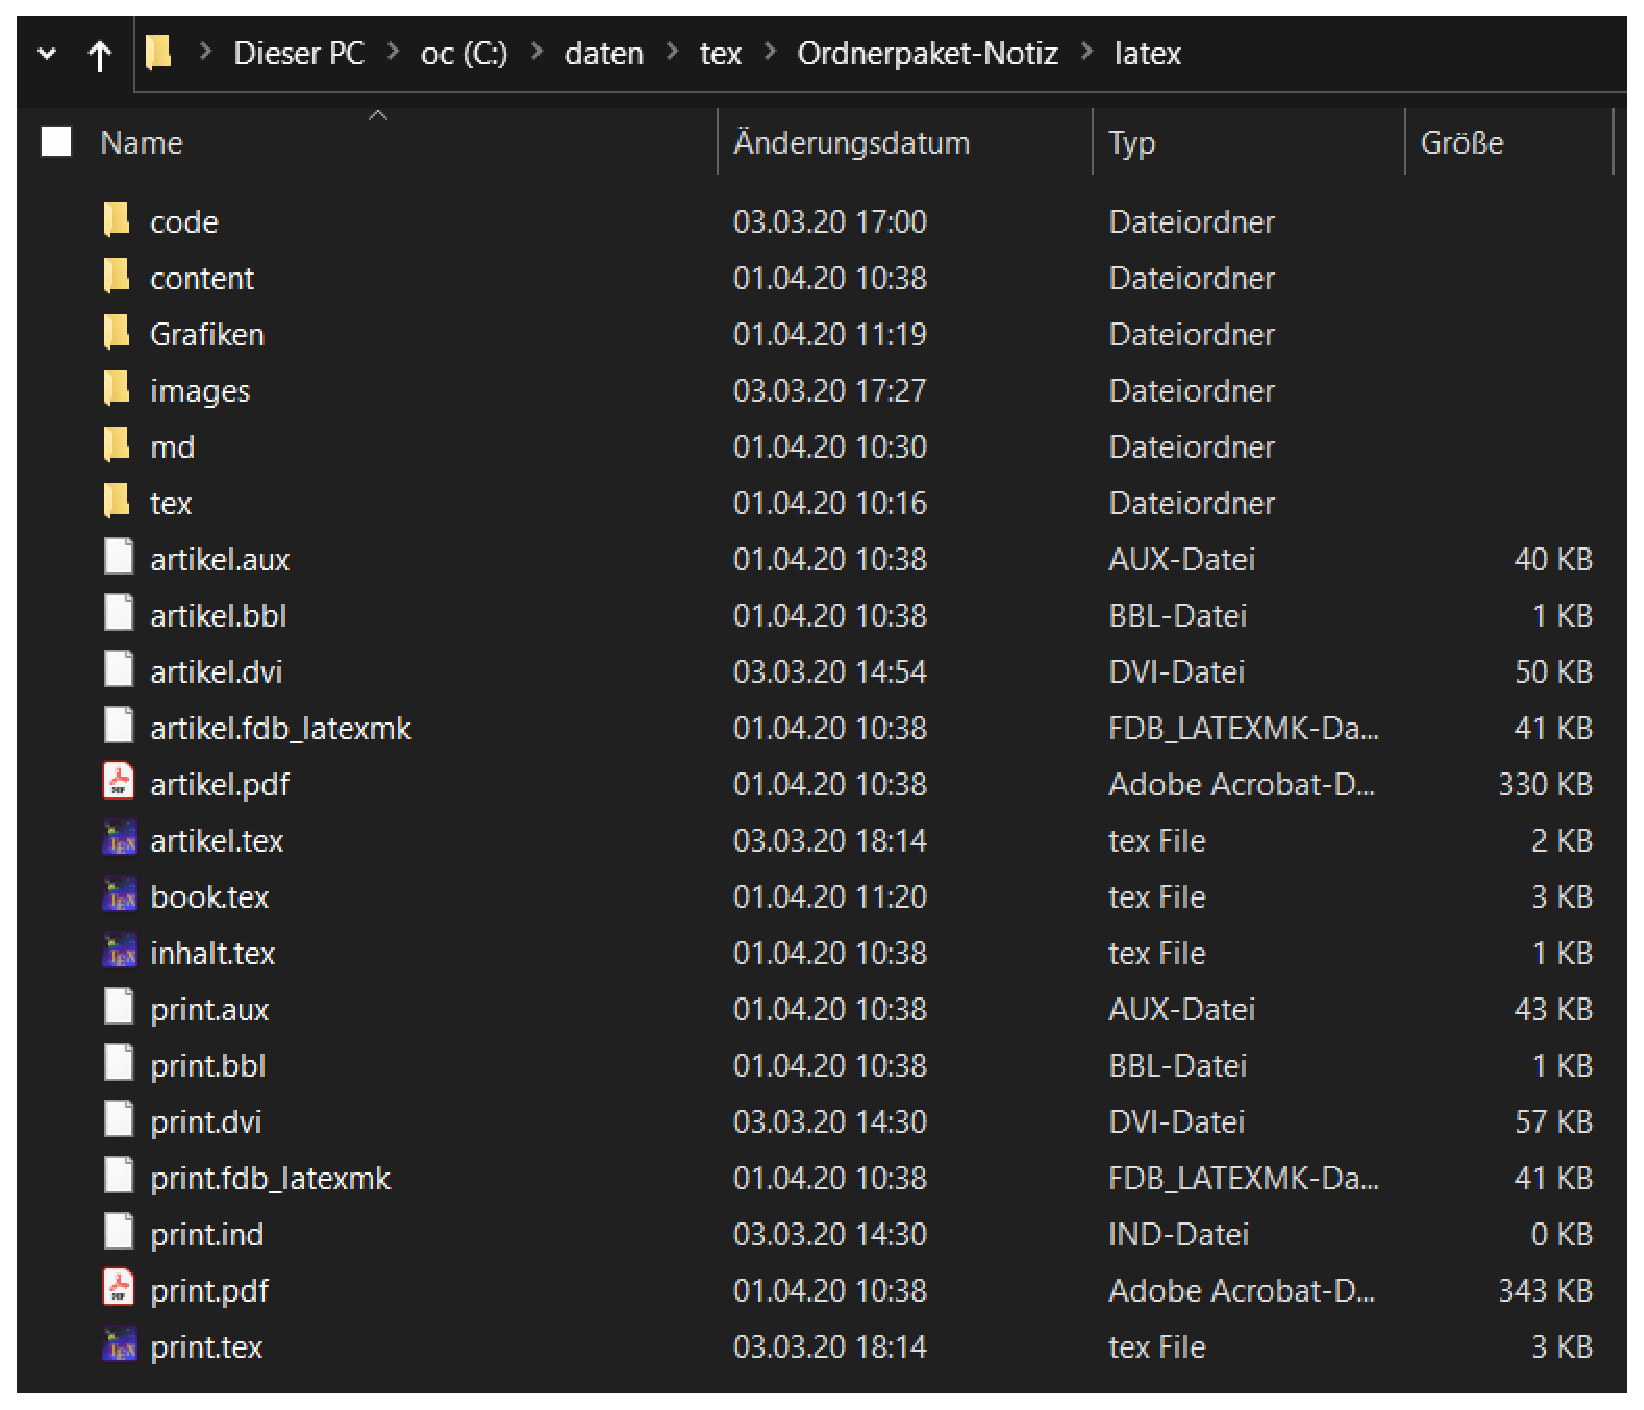
\includegraphics[width=0.7\textwidth]{images/ordner-latex}
  \caption{ordner-latex}%  Name
  \label{fig:ordner-latex}% Ref.
\end{figure}
  

>>ordner-struktur<< (vgl. Abb.~\ref{fig:ordner-struktur}).% Referenz
  % Abb.
\begin{figure}[H]% hier: hbtp 
  \centering
  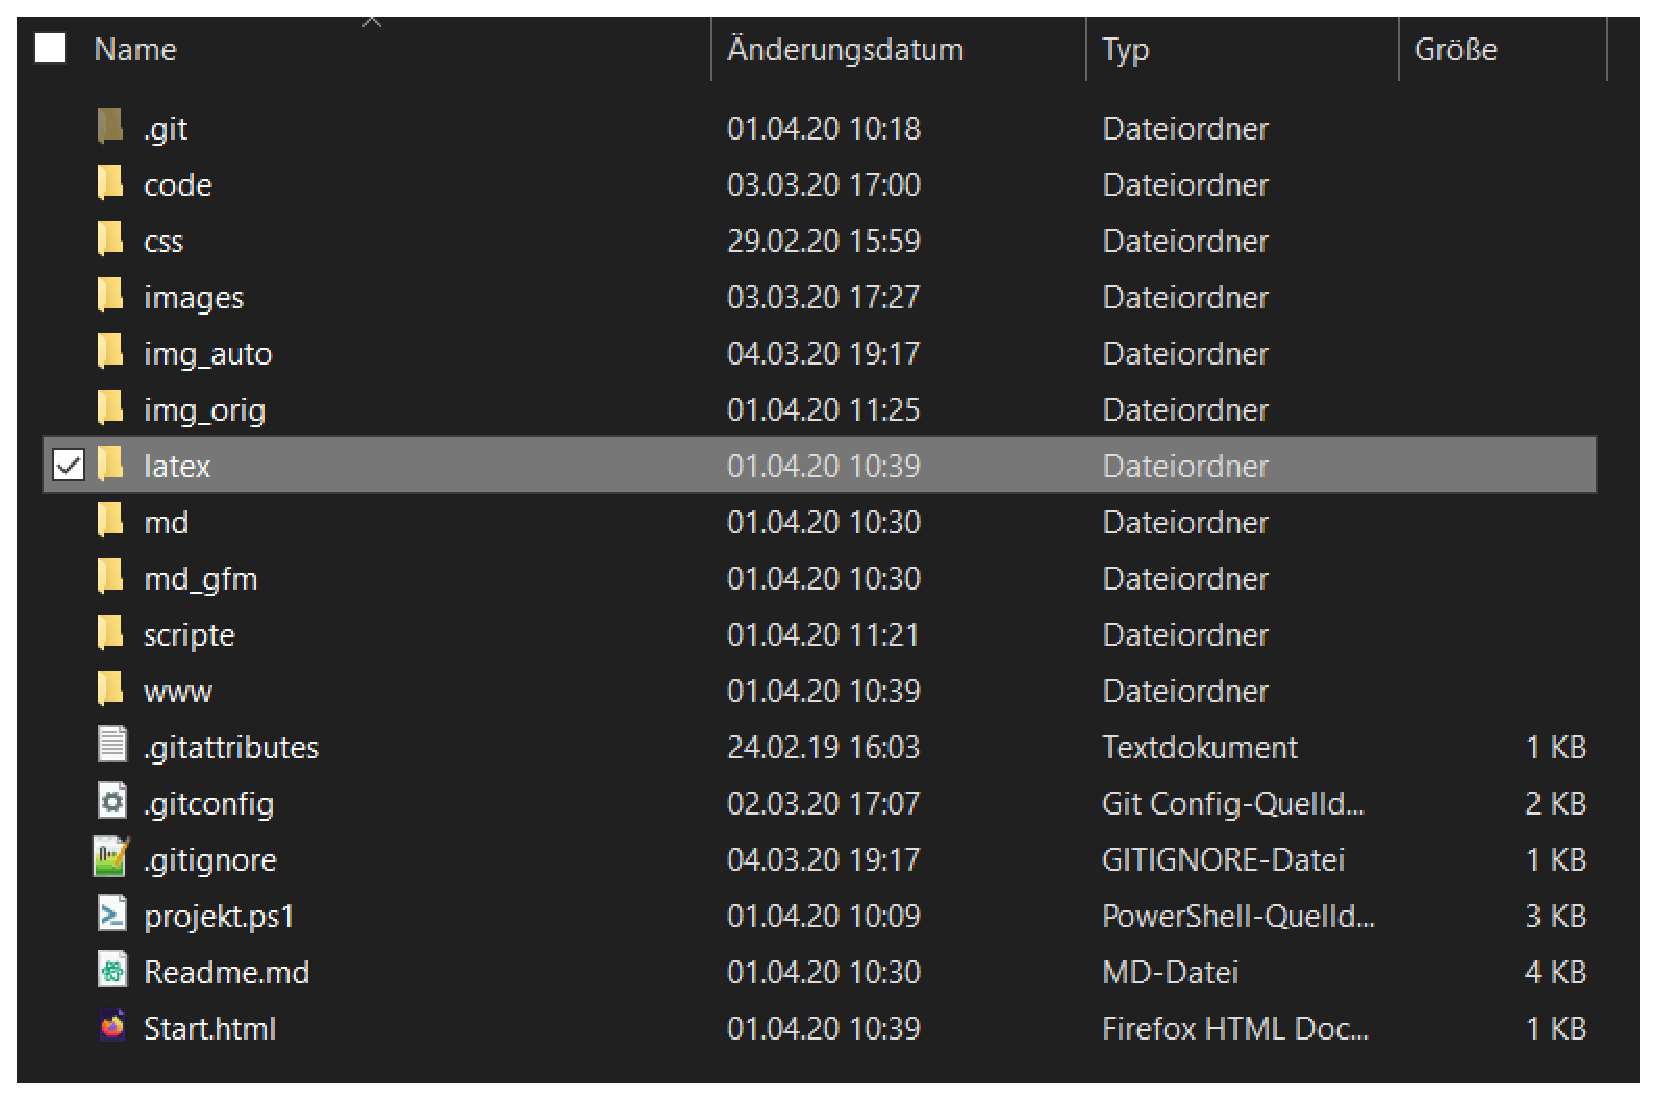
\includegraphics[width=0.7\textwidth]{images/ordner-struktur}
  \caption{ordner-struktur}%  Name
  \label{fig:ordner-struktur}% Ref.
\end{figure}
  

>>Sport-Kraft<< (vgl. Abb.~\ref{fig:Sport-Kraft}).% Referenz
  % Abb.
\begin{figure}[H]% hier: hbtp 
  \centering
  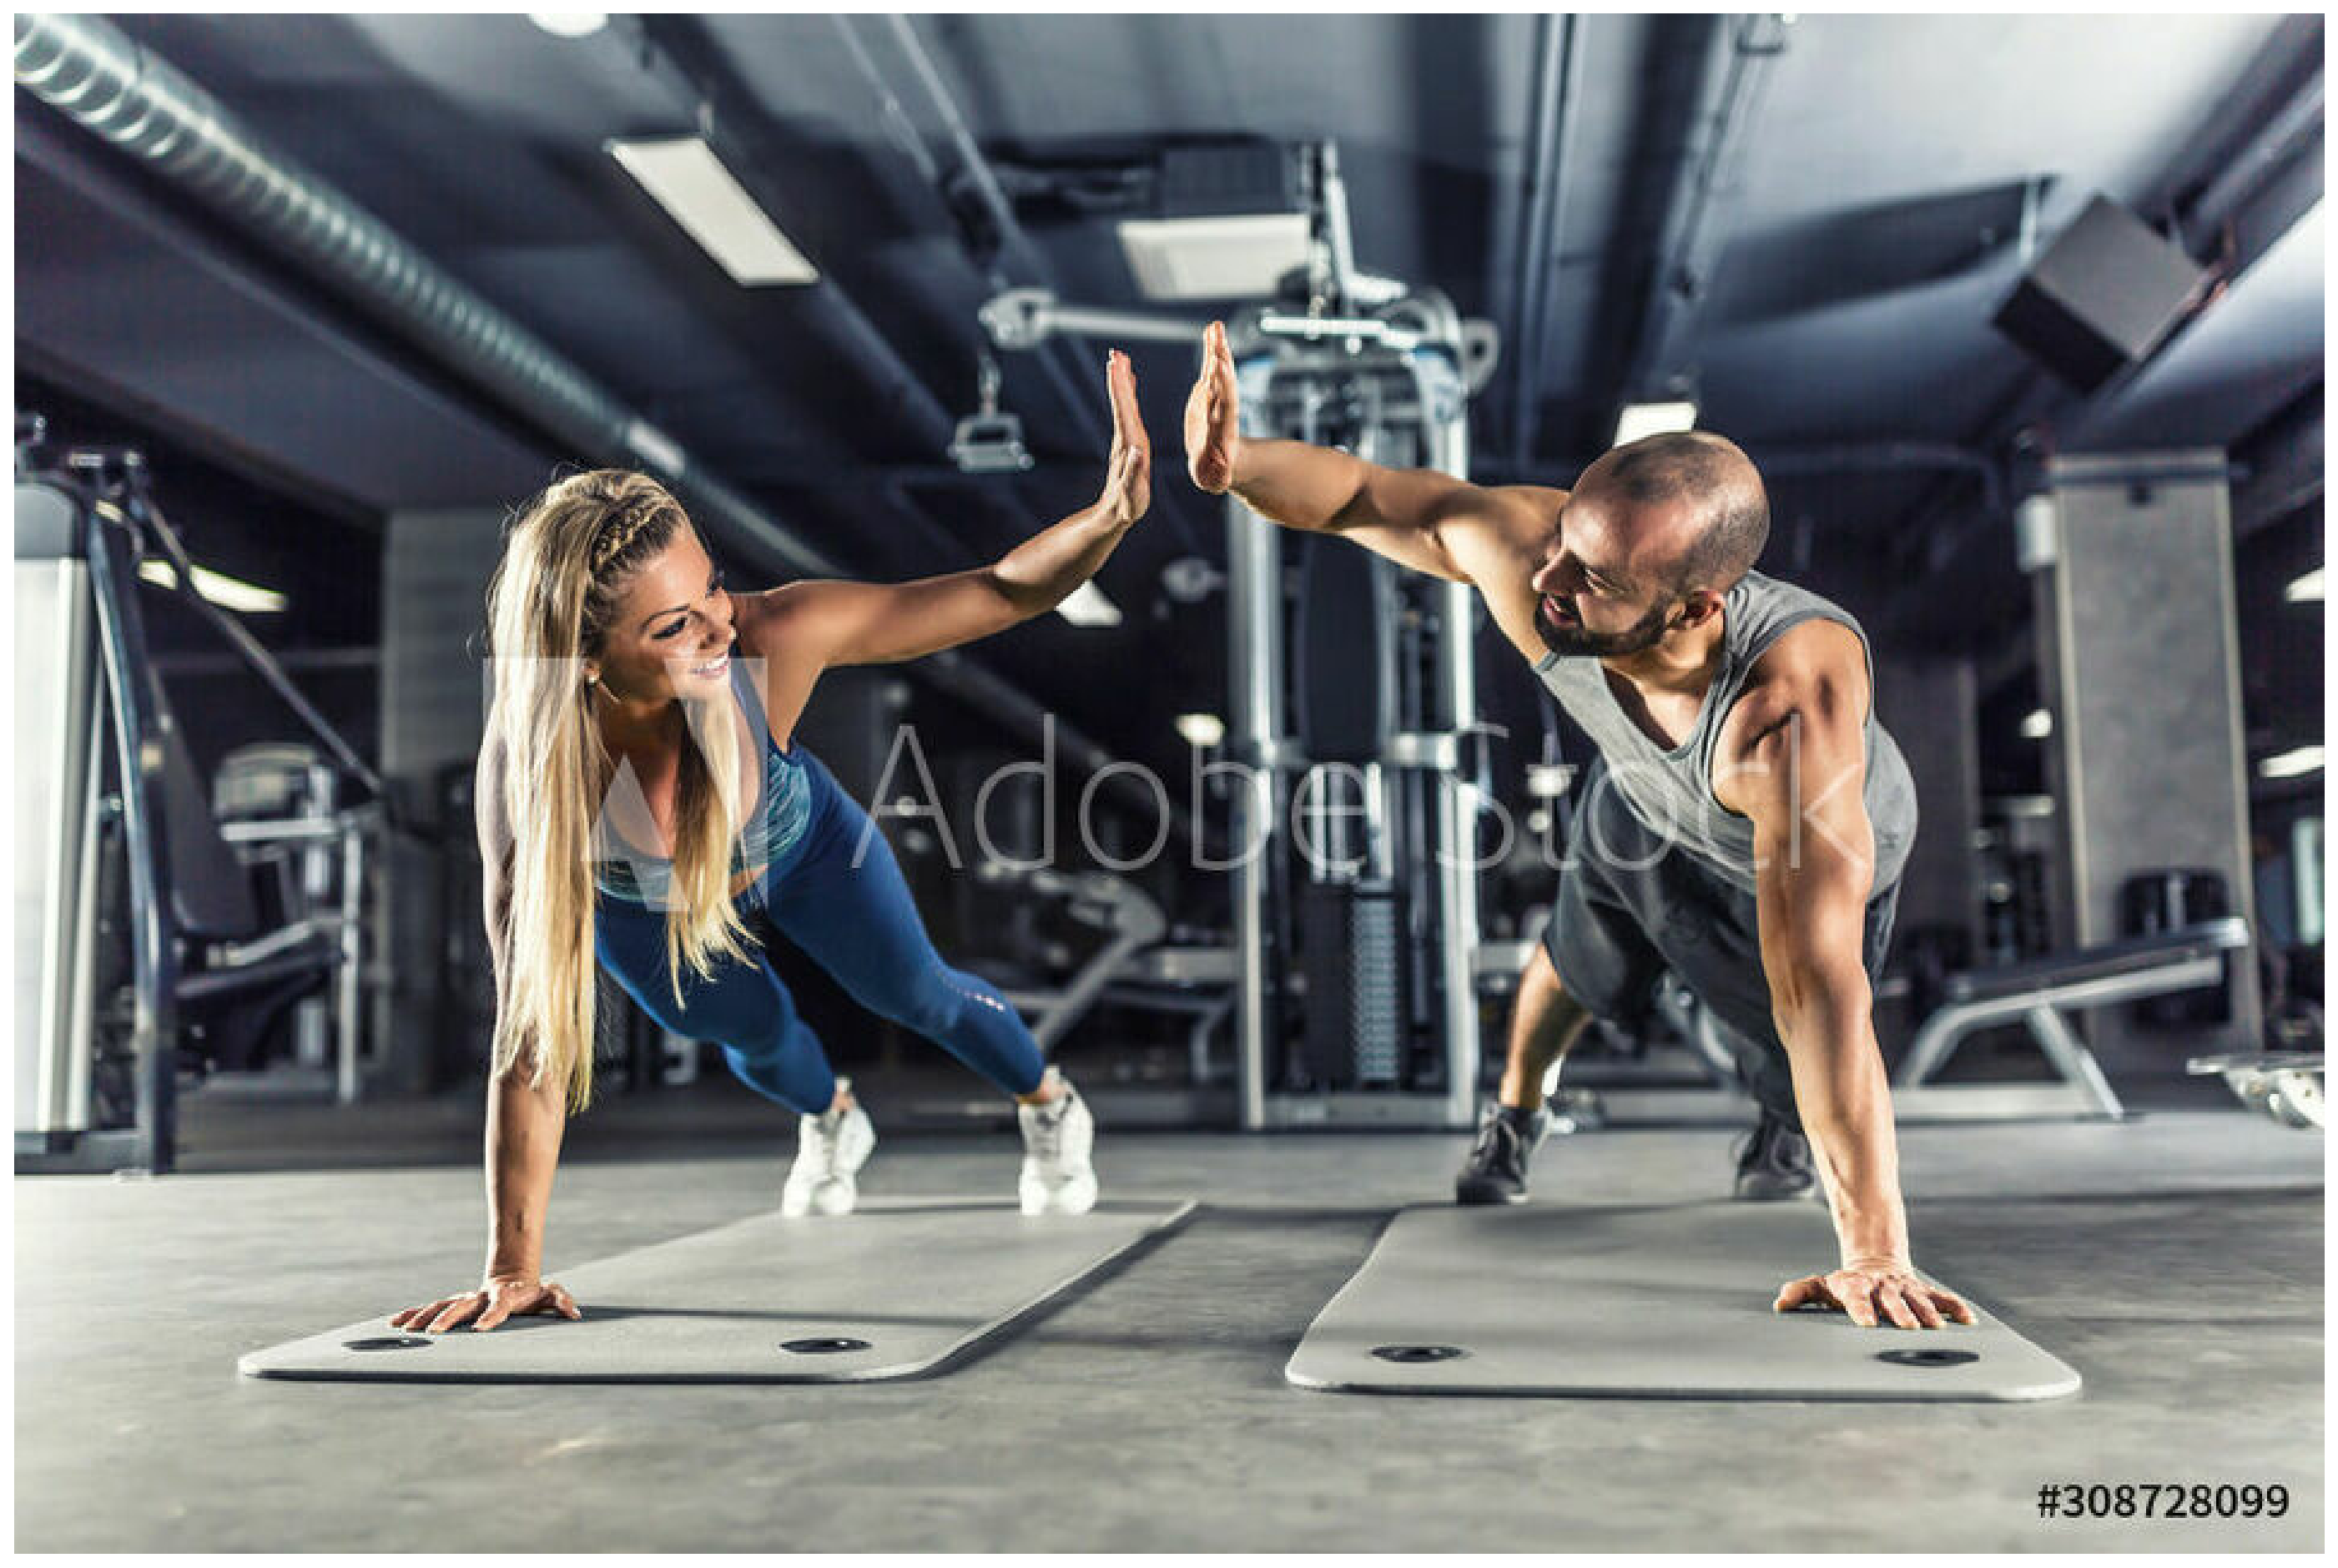
\includegraphics[width=0.7\textwidth]{images/Sport-Kraft}
  \caption{Sport-Kraft}%  Name
  \label{fig:Sport-Kraft}% Ref.
\end{figure}
  

>>Sport-Winter<< (vgl. Abb.~\ref{fig:Sport-Winter}).% Referenz
  % Abb.
\begin{figure}[H]% hier: hbtp 
  \centering
  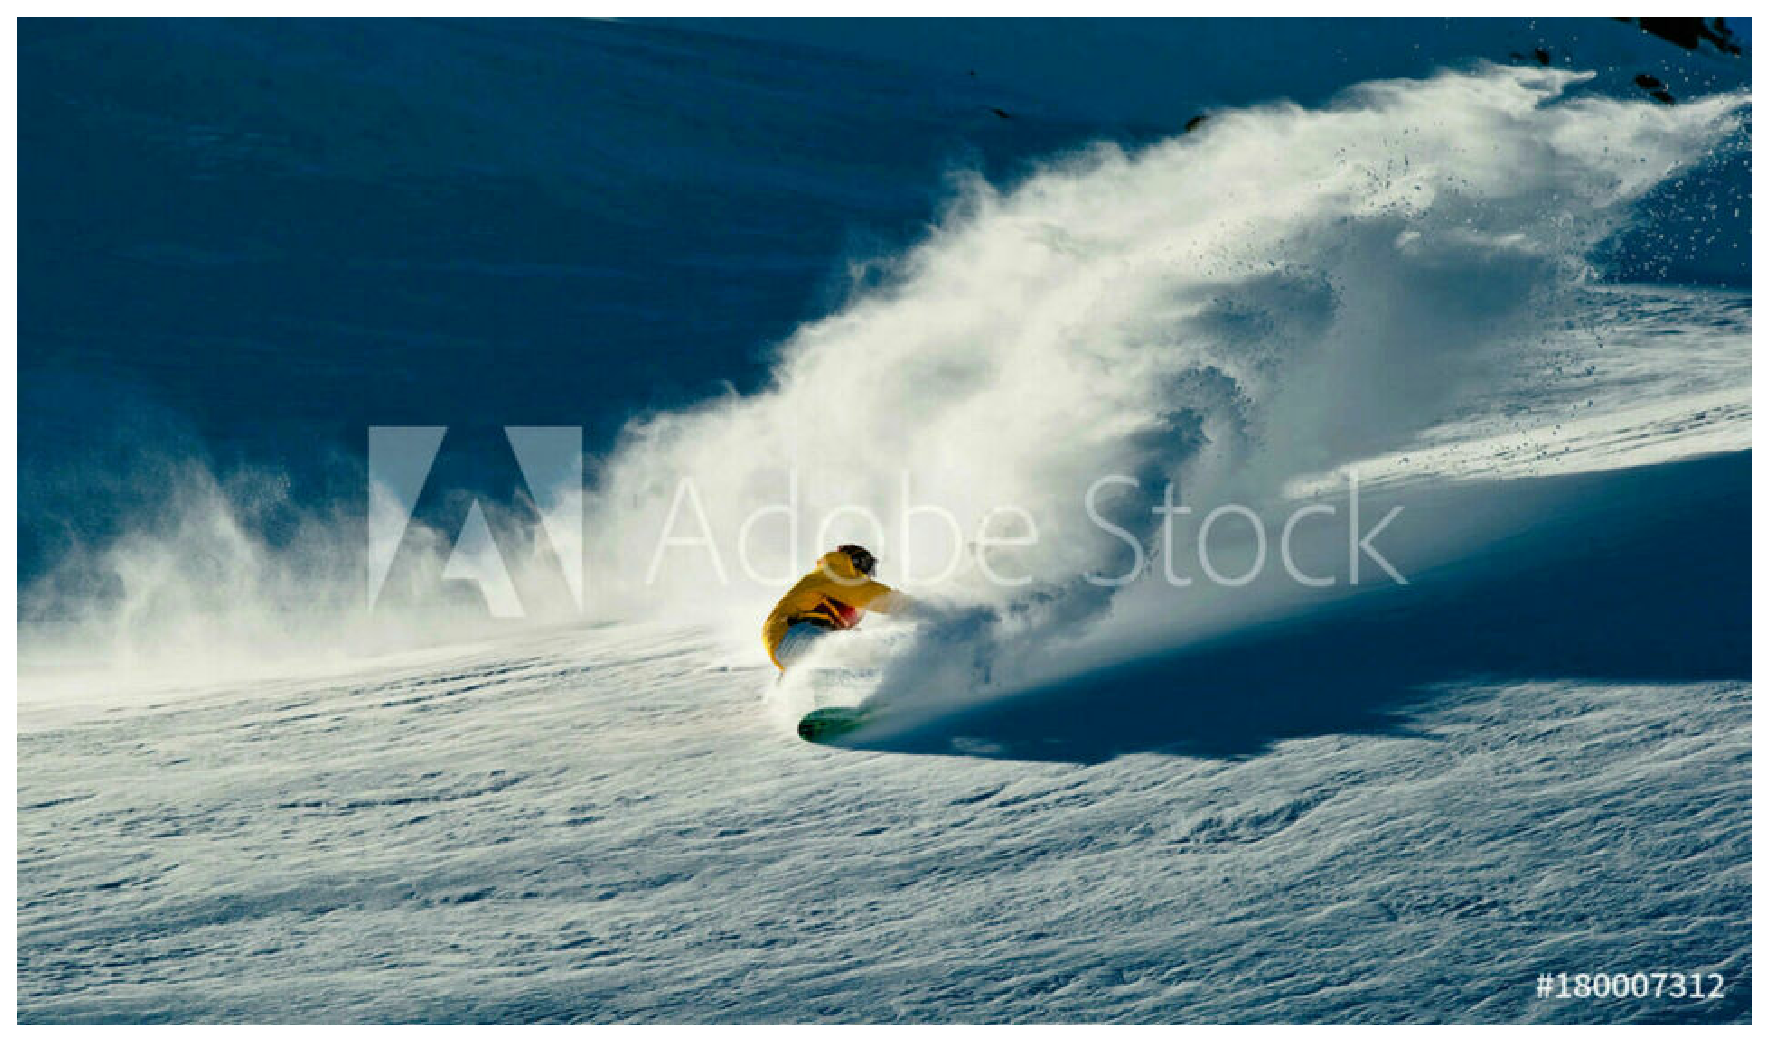
\includegraphics[width=0.7\textwidth]{images/Sport-Winter}
  \caption{Sport-Winter}%  Name
  \label{fig:Sport-Winter}% Ref.
\end{figure}
  


